\documentclass[11pt,a4paper,oneside]{article}
\usepackage[utf8]{inputenc}
\usepackage[french]{babel}
\usepackage[T1]{fontenc}
\usepackage{graphicx}
\usepackage{charter}
\usepackage{hyperref}
\usepackage[left=2cm,right=2cm,top=2cm,bottom=2cm]{geometry}
\author{Mylann Dupuy}
\title{Rapport de stage}
\begin{document}
\maketitle
\newpage
\tableofcontents
\newpage
\section{Contexte}
Le centre Jean Bernard / Clinique Victor Hugo voudrait mettre un nouveau système de déploiement pour déployer diverses logiciels.
\section{Objectif(s)}
L'objectif est de déployer les logiciels utilisés couramment et de les mettre à jour. Le système doit fonctionner avant la fin du stage. 
\subsection{Cahier des charges}
\begin{itemize}
	\item Adobe Flash Player 24
	\item Adobe Reader DC
	\item Java 8 Update xx
	\item Mozilla Firefox
	\item Mozilla Thunderbird
	\item PDFCreator
	\item 7-Zip
\end{itemize}
Tout les logiciels doivent êtres installés avec des paramètres spécifiques !
\\
\subsection{Contraintes}
Lors du déploiement, les Postes sont constamment utilisé par le personnel du centre. Pour pouvoir intervenir, il faut appelé la personne présente sur le Poste et intervenir à distance avec \textbf{TightVNC}.
\subsection{Matériels disponible}
\begin{itemize}
	\item \textbf{1 Ordinateur} pour administrer et surveiller OCS.
	\item \textbf{1 Serveur virtuel} sous 	\textbf{Debian 8.7}.
	\item \textbf{1 Serveur de stockage}  pour l'accès aux exécutables prévus pour les scripts. 

\end{itemize}
\newpage
\section{Solutions}
\subsection{Comparaison}
En farfouillant sur Internet et aussi avec mes connaissances personnelles, j'ai recensé 5 solutions de déploiement mais dans notre contexte, il y a 2 solutions qui seront comparées \\ \\
%%%%%%%%%%%%%%%%%%%%%%%%%%%%%%%%%%%%%%%%%%%%%%%%%%%%%%%%%%%%%%%%%%%%%%%%%%%%%%%%%%%%%%%%%%%%%%%%%%%%%%%%%%%%%%%
\begin{tabular}{|p{3.1cm}|p{6.5cm}|p{6.5cm}|}
	\hline
	\centering Solutions : & \centering Avantages : & Inconvénients : \\
	\hline
	%%%%%%%%%%%%%%%%%%%%%%%%%%%%%%%%%%%%%%%%%%%%%%%%%%%%%%%%%%%%%%%%%%%%%%%%%%%%%%%%%%%%%%%%%%%%%%%%%%%%%%%%%%%
	\centering OCS Inventory NG  & \begin{itemize}
							\item Faible utilisation de la bande passante 
							\item Plugins pour GLPI							
							\item Supervision des logiciels installé
							\item Logiciel libre disponible sous Windows Server / Client
							\item Inventaire complet des Postes							
						\end{itemize} & \begin{itemize}
												\item Wiki non à jour  
												\item Paquets Debian en version 2.0.5																			\end{itemize} \\
	\hline
	%%%%%%%%%%%%%%%%%%%%%%%%%%%%%%%%%%%%%%%%%%%%%%%%%%%%%%%%%%%%%%%%%%%%%%%%%%%%%%%%%%%%%%%%%%%%%%%%%%%%%%%%%%%
	\centering WAPT  & \begin{itemize}
							\item Automatisation d'installation, MAJ et suppressions logiciels 
							\item Centralisation graphique du déploiement
							\item Facilité pour les MAJ 
							\item Gestion des dépendances
							\item Logiciel libre													
						\end{itemize} & \begin{itemize}
												\item Configuration à faire pour faire cohabiter WSUS et WAPT 
												\item Packages propre à WAPT (.wapt)
												\item Suite Microsoft Office non Disponible
												\item Supervision des logiciels installé
												\item Création de paquets + ou - complèxe
												\item Certains logiciels ne sont plus à jour			
										\end{itemize} \\
	\hline	
\end{tabular}
%%%%%%%%%%%%%%%%%%%%%%%%%%%%%%%%%%%%%%%%%%%%%%%%%%%%%%%%%%%%%%%%%%%%%%%%%%%%%%%%%%%%%%%%%%%%%%%%%%%%%%%%%%%%%%
\\ \\
Nous avons décidés de mettre en place \textbf{OCS Inventory NG 2.3} (cf.Références) car les logiciels qui doivent être déployer seront facilement mis à jour contrairement à WAPT.
\\
\subsection{Mise en \oe{}uvre}
\subsubsection{Avant de commencer} 
Nous avons créer une machine virtuelle sous Hyper-V (cf.Références) en lui mettant comme ressources :\\ \begin{itemize}
				\item 1 image ISO de Debian 8.7
				\item 4 Go de mémoire vive
				\item 1 C{\oe}ur du processeur
				\item 50 Go d'espace disque
				\item 1 connexion au réseau CJB	
\end{itemize} 

\begin{center}
\textbf{Cette configuration est hébergée sur le Poste de M.Deshayes}
\end{center}
\newpage
\subsubsection{Installation}
Lors de l'installation, j'ai tout laissé par défaut sauf le proxy qui à été renseigné. Suite à l'installation, j'ai eu à installer \textbf{openssh-server} pour tout faire via \textbf{PuTTY}.\\

Depuis SSH, il fallait installer un serveur Web, un serveur BDD, PHP, Perl et leurs modules (\textbf{apache2, mylsql-server, php5, perl, libxml-simple-perl, libcompress-zlib-perl, libdbi-perl libdbd-mysql-perl,libapache-dbi-perl, libnet-ip-perl, libsoap-lite-perl}). Pour les modules Perl en cas de problèmes de paquets, il faut les télécharger et les installer à la main depuis ce site \url{http://search.cpan.org/} \\

S'il manque des paquets, le script d'installation d'OCS Inventory les installera mais dans notre cas, on est derrière un proxy donc vaut mieux tout installer avant. \\

Pour installer OCS Inventory NG, j'ai utilisé l'archive qui était sur le site via  et la documentation non à jour.
\newpage
\section{Principe de fonctionnement}
\begin{figure}[hbtp]
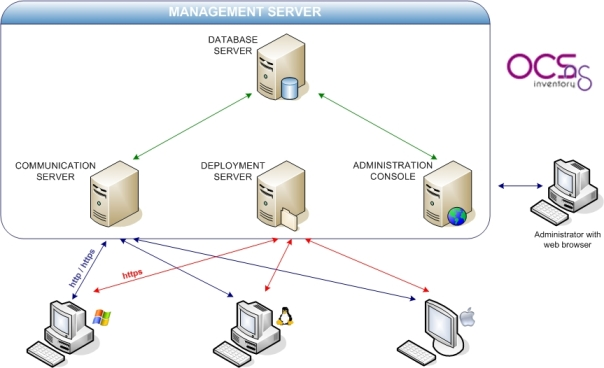
\includegraphics[scale=0.8]{../../../Downloads/deploy.jpg}
\caption{Schéma de déploiement}
\end{figure}
L'architecture reste simple à mettre en place, dans l'environnement actuel nous avons tout mis sur le même serveur.
\subsection{Outil de déploiement}
\begin{figure}[hbtp]
\centering
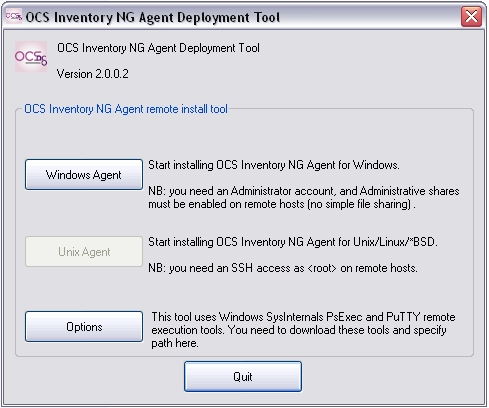
\includegraphics[scale=0.5]{../../../Pictures/Script/1.jpg}
\caption{Etape 1 - Écran de démarrage}
\end{figure}
Avant de faire le déploiement de logiciels sur le réseau, il faut installer l'agent OCS sur les Postes Clients avec \textbf{OCS Inventory NG Agent Deployment Tool} puis aussi vérifier si les partages administratifs (C\$) sont bien activés puis passer à \textbf{l'étape 2}.
\newpage

\begin{figure}[hbtp]
  \centering
  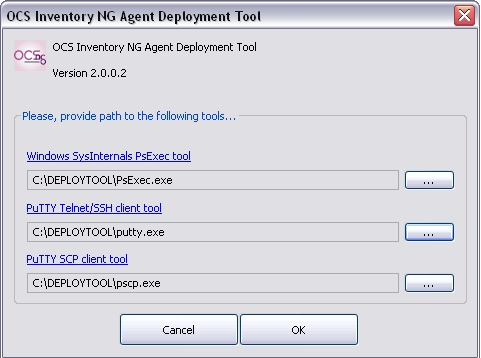
\includegraphics[scale=0.5]{../../../Pictures/Script/2.jpg}
  \caption{Etape 2 - La configuration de l'outil de déploiement}
\end{figure} 
Dans notre cas, il faut déployer l'agent sur les Postes Clients mais pour ce faire, il faut utilisé le module PSEXEC (cf.Références) depuis le Poste qui va déployer l'agent OCS. Il suffit de mettre le répertoire exacte du module précédemment télécharger depuis le site dans les options d'OCS Inventory NG Agent Deployment Tool. Quand c'est fait, il faut passer à \textbf{l'étape 3}. \\

\begin{figure}[hbtp]
 \centering
 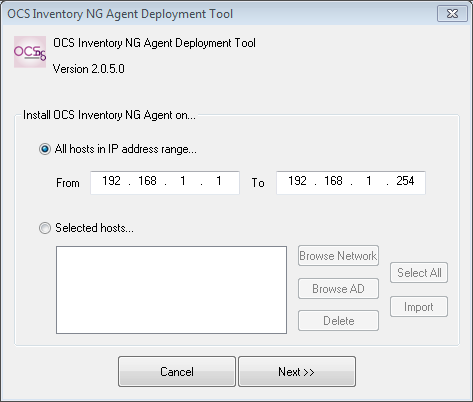
\includegraphics[scale=0.7]{../../../Pictures/Script/3.png}
 \caption{Etape 3 - La sélection des Postes}
 \end{figure}
  
\textbf{l'étape 3} consiste à définir une plage IP  ou à selectionner le(s) Poste(s) qui auront l'agent OCS. Dans notre cas, on avait défini une plage IP sur l'ensemble du réseau CJB. Après la selection des Postes, on passe à \textbf{l'étape 4}.
\newpage

\begin{figure}[hbtp]
\centering
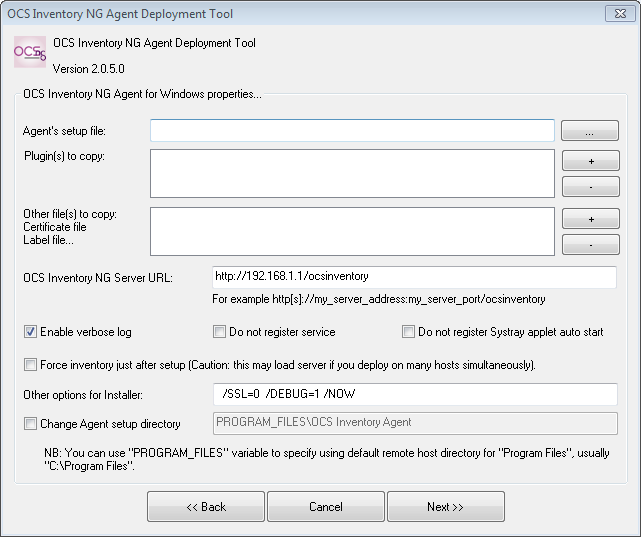
\includegraphics[scale=0.7]{../../../Pictures/Script/4.png}
\caption{Etape 4 - Les paramètres de l'agent OCS}
\end{figure}

C'est à partir de là qu'on va faire la configuration de l'agent OCS qui sera mis en place lors du déploiement.  
\begin{enumerate}
\item Il faut lui donner le répertoire où se trouve le fichier d'installation de l'agent.
\item Les plugins ou fichier à copier sur le Poste Client.
\item Le certificat du serveur si SSL est activé sur le serveur OCS.
\item L'adresse URL du serveur OCS.
\item Activer les options pour l'agent OCS (Logs, Ne pas enregistrer en tant que service, Ne pas mettre l'icone dans la barre de notifications au démarrage du Poste, Forcer l'inventaire après l'installation).
\item Les options spécifiques qu'on veut mettre. Les options choisies au dessus sont écrites dans cet encadrement.
\item Le répertoire d'installation pour l'agent OCS sur le(s) Poste(s) Client(s).
\end{enumerate}
Quand cette étape est faite en ayant bien vérifier avant, on passe à \textbf{l'étape 5} qui terminera les étapes de configuration de l'agent.
\newpage
\begin{figure}[hbtp]
\centering
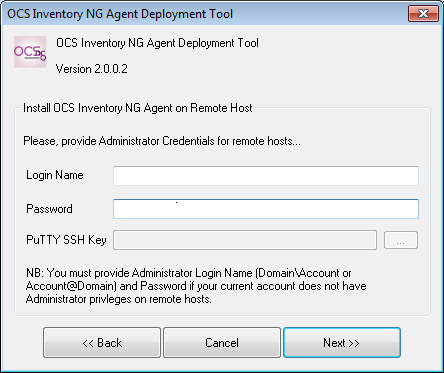
\includegraphics[scale=0.9]{../../../Pictures/Script/5.png}
\caption{Etape 5 - L'authentification}
\end{figure}

Pour permettre le déploiement de l'agent OCS SANS déranger les utilisateurs ni en intervenant sur les Postes Clients, il faut renseigner les informations de connexion du compte "Administrateur" du domaine pour les Postes WINDOWS. Si les informations sont exactes, on lance le déploiement à l'étape 6.

\begin{figure}[hbtp]
\centering
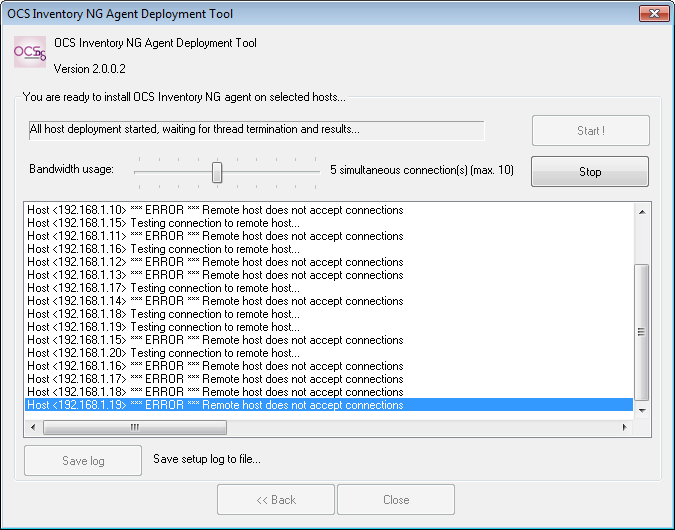
\includegraphics[scale=0.6]{../../../Pictures/Script/6.png}
\caption{Etape 6 - Log de déploiement}
\end{figure}

Après avoir tout bien fait, il suffit de lancer le déploiement pour qu'il installe l'agent OCS sur les Postes Clients. L'outil de déploiement peut déployer les Postes Clients 1 par 1 ou peut faire 10 connexions simultanées, c'est-à-dire qu'il va faire l'operation sur 10 postes maximum. \\ 
\textbf{ATTENTION ! En changeant le nombre de connexion simultanées, on augmente la charge du CPU.}
\newpage
\subsection{Interface Web OCS Inventory}
Lors que l'agent est bien installé sur les Postes Clients, il doivent faire l'inventaire complet de la machine et envoyer automatiquement l'inventaire au serveur. Suite à ça, on peut se faire une idée sur les logiciels qu'on doit déployer ou non. \\

En arrivant sur l'écran d'inventaire, on remarque les différentes informations sur les Postes Clients (TAG, Dernier Inventaire, Le nom de l'ordinateur, L'utilisateur actuel, OS, Fréquences RAM / CPU) qui sont automatiquement inventoriés selon la configuration faite depuis le serveur.

 
%Résumé d'utilisation d'OCS
% Utilisation du Module de déploiement
bla bla
\section{Résultat Final}
bla bla
\subsection{Problèmes rencontrés}
bla bla
\section{Conclusion}
bla bla
\section{Annexes}

\section{Références}

Microsoft Hyper-V :
\\
OCS Inventory NG 2.3 :\url{www.ocsinventory-ng.org/fr/}
\\
Wiki d'OCS Inventory :\url{http://wiki.ocsinventory-ng.org/index.php?title=Documentation:Server/fr}
\\
OCS Inventory NG Agent Deployment Tool :
\\
PSEXEC :
\end{document}